\chapter{अम्ल--क्षारक साम्य और प्रधान-अभिक्रिया विधि}\label{ch:b1:predominant-reaction}

सिरका केतली की पपड़ी (चूने की परत) घोल देता है; नींबू का रस भी, थोड़ा और
तेज़ी से। हम चाहे जो खाएँ, रक्त अपना pH संकरी सीमाओं में बनाए रखता है;
सोडा-पेय अपने भीतर घुली कार्बन डाइऑक्साइड के कारण अम्लीय होता है। ये सब
पानी में अम्ल--क्षारक साम्य हैं, और जिस रसायनज्ञ के सामने कई अम्लों और क्षारकों
वाला विलयन हो --- कोई मिश्रण, कोई बफ़र, कोई \omterm{def:b1:predominant-reaction:polyprotic}{बहुप्रोटिक अम्ल} --- उसे उसका pH
और उसकी स्पीशीज़ की सांद्रताएँ ज्ञात करने का एक विश्वसनीय तरीका चाहिए। यह अध्याय वह
विधि बनाता है: प्रबलताओं का एक पैमाना, \omterm{def:b1:predominant-reaction:predominance}{प्रभाविता आरेख}, और \emph{प्रधान-अभिक्रिया
विधि}, जो किसी भी मिश्रण को उस एक अभिक्रिया तक घटा देती है जो मायने रखती है।

\begin{recall}
पुस्तक 1 (कक्षा 12) ने \omterm{def:b1:predominant-reaction:bronsted}{ब्रॉन्स्टेड अम्लों} और क्षारकों, \omterm{def:b1:predominant-reaction:acidity-constant}{अम्लता स्थिरांक}
$K_a$ और $\mathrm{p}K_a$, \omterm{def:b1:predominant-reaction:autoprotolysis}{जल के आयनिक गुणनफल} और \omterm{def:b1:predominant-reaction:strong-acid}{प्रबल
अम्लों} और क्षारकों के pH को परिभाषित किया था, और \omterm{def:b1:predominant-reaction:predominance}{प्रभाविता आरेख} बनाए थे। \omterm{def:b1:extent-q-and-k:quotient}{अभिक्रिया भागफल},
साम्य स्थिरांक और विलेयों ($c/c^\circ$) तथा
विलायक (1) की \omterm{def:b1:extent-q-and-k:activity}{सक्रियताएँ} \cref{ch:b1:extent-q-and-k} में परिभाषित की गईं; इस
अध्याय में भागफलों में $c^\circ = \qty{1}{mol/L}$ नहीं लिखा जाता।
\end{recall}

\begin{omfigure}
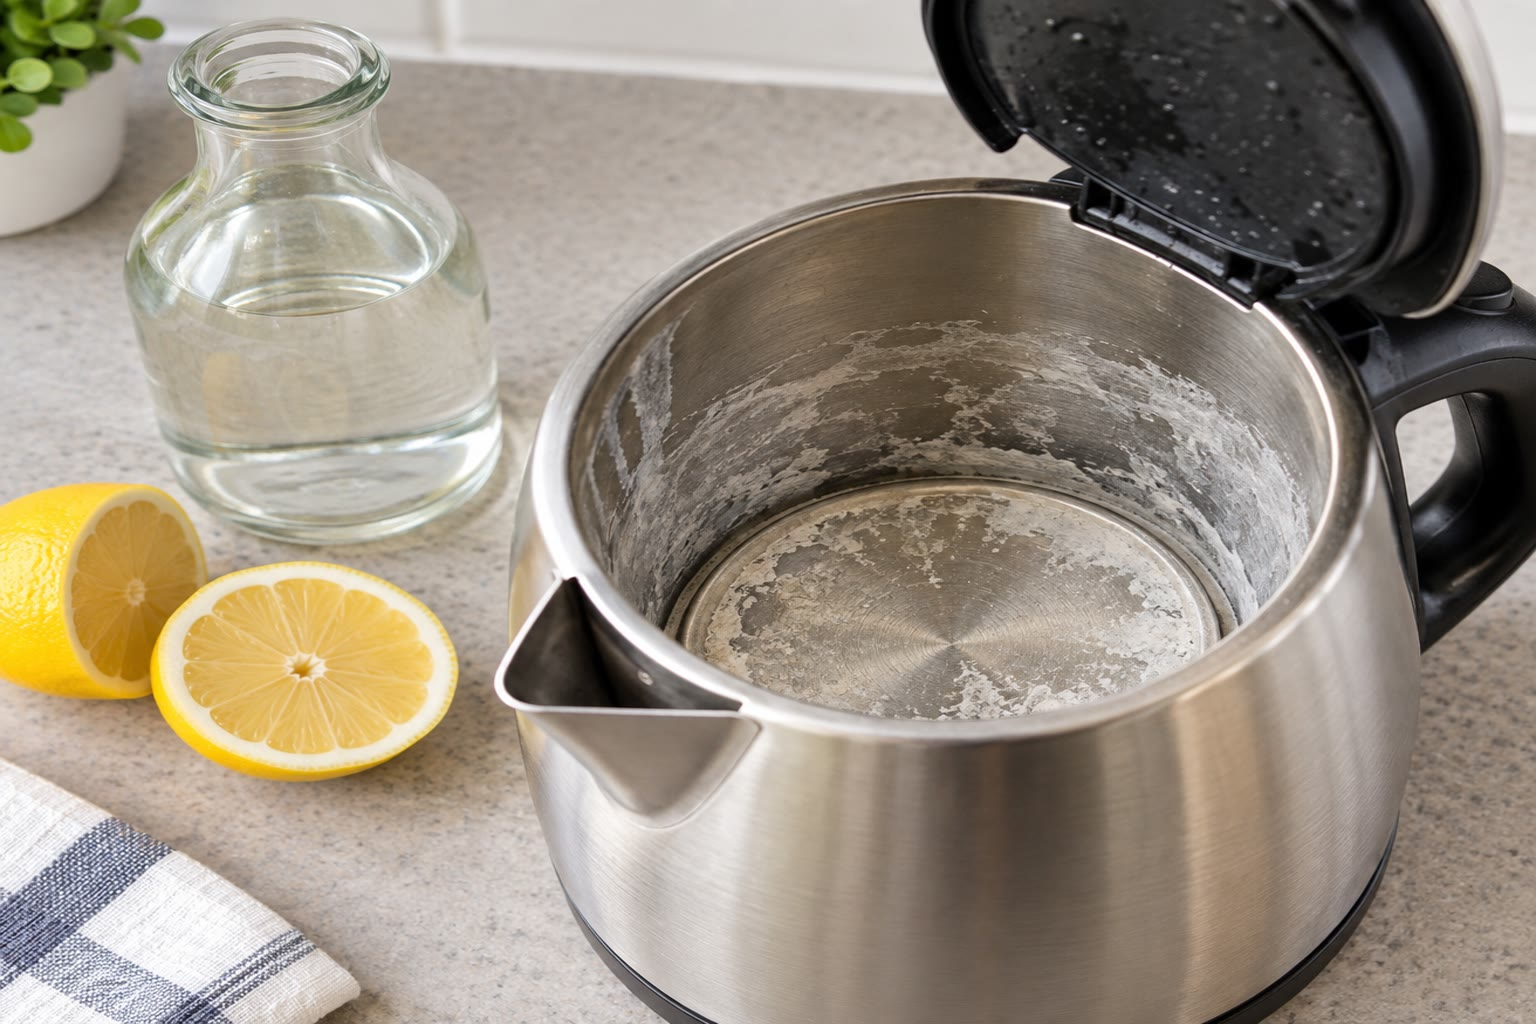
\includegraphics[width=0.5\linewidth]{images/book2/ai/b1-10-descaling.jpg}

{\small केतली में चूने की पपड़ी, कैल्सियम कार्बोनेट। सिरके और नींबू के रस के
\omterm{def:b1:predominant-reaction:strong-acid}{दुर्बल अम्ल} कार्बोनेट आयन से अभिक्रिया करके उसे घोल देते हैं।}
\end{omfigure}

\section{ब्रॉन्स्टेड युग्म और pH}

\begin{definition}[ब्रॉन्स्टेड अम्ल और क्षारक, युग्म]\label{def:b1:predominant-reaction:bronsted}
\emph{ब्रॉन्स्टेड अम्ल}\index{ब्रॉन्स्टेड अम्ल} वह स्पीशीज़ है जो
प्रोटॉन \ce{H+} दे सकती है; \emph{ब्रॉन्स्टेड क्षारक}\index{ब्रॉन्स्टेड क्षारक} वह स्पीशीज़ है
जो प्रोटॉन ग्रहण कर सकती है। कोई अम्ल HA और वह क्षारक A जो यह अम्ल एक प्रोटॉन खोकर बनता है,
एक \emph{अम्ल--क्षारक युग्म}\index{अम्ल--क्षारक युग्म} HA/A बनाते हैं,
जो औपचारिक अर्ध-समीकरण $\mathrm{HA} \rightleftharpoons
\mathrm{A} + \ce{H+}$ से संबद्ध हैं। पानी में प्रोटॉन कभी मुक्त नहीं होता: उसे
पानी का एक अणु \ce{H3O+} के रूप में वहन करता है।
\end{definition}

\begin{definition}[उभयधर्मी]\label{def:b1:predominant-reaction:ampholyte}
\emph{उभयधर्मी}\index{उभयधर्मी} (उभयधर्मी स्पीशीज़) एक युग्म का क्षारक
और दूसरे युग्म का अम्ल होता है: पानी (\ce{H3O+}/\ce{H2O} और
\ce{H2O}/\ce{OH-}), हाइड्रोजनकार्बोनेट आयन (\ce{CO2,H2O}/\ce{HCO3-}
और \ce{HCO3-}/\ce{CO3^{2-}}), डाइहाइड्रोजनफ़ॉस्फ़ेट आयन।
\end{definition}

\begin{definition}[स्वप्रोटॉनी अपघटन, आयनिक गुणनफल, pH]\label{def:b1:predominant-reaction:autoprotolysis}
पानी में \emph{स्वप्रोटॉनी अपघटन}\index{स्वप्रोटॉनी अपघटन} होता है,
\ce{2H2O <=> H3O+ + OH-}, जिसका स्थिरांक $K_e = [\ce{H3O+}][\ce{OH-}]$
\emph{जल का आयनिक गुणनफल}\index{जल का आयनिक गुणनफल} है;
\qty{25}{\celsius} पर $K_e = 10^{-14.00}$, इसलिए $\mathrm{p}K_e = 14.00$। किसी विलयन का pH
$\mathrm{pH} = -\log a(\ce{H3O+}) \approx -\log[\ce{H3O+}]$ है।
विलयन उदासीन होता है जब $[\ce{H3O+}] = [\ce{OH-}]$, अर्थात्
\qty{25}{\celsius} पर $\mathrm{pH} = \mathrm{p}K_e/2 = 7.00$ पर।
% ledger: dfg:H2O_l, dfg:OH-_ao (pKe computed in figdata/bachelor-1/aqueous-constants.py)
\end{definition}

\section{प्रबलता: \texorpdfstring{$K_a$}{Ka}, \texorpdfstring{p$K_a$}{pKa} और समतलन प्रभाव}

\begin{definition}[अम्लता स्थिरांक]\label{def:b1:predominant-reaction:acidity-constant}
किसी युग्म HA/A का \emph{अम्लता स्थिरांक}\index{अम्लता स्थिरांक}
पानी के साथ अम्ल की अभिक्रिया का स्थिरांक है,
\[
  \mathrm{HA} + \ce{H2O} \rightleftharpoons \mathrm{A} + \ce{H3O+}, \qquad
  K_a = \frac{[\mathrm{A}][\ce{H3O+}]}{[\mathrm{HA}]}, \qquad
  \mathrm{p}K_a = -\log K_a .
\]
$K_a$ जितना बड़ा (और $\mathrm{p}K_a$ जितना छोटा), अम्ल उतना \omterm{def:b1:predominant-reaction:strong-acid}{प्रबल} और
उसका संयुग्मी क्षारक उतना \omterm{def:b1:predominant-reaction:strong-acid}{दुर्बल}।
\end{definition}

\begin{definition}[प्रबल और दुर्बल अम्ल और क्षारक]\label{def:b1:predominant-reaction:strong-acid}
पानी में कोई अम्ल \emph{प्रबल}\index{प्रबल अम्ल} होता है यदि पानी के साथ उसकी
अभिक्रिया पूर्ण हो: कोई अणु HA शेष नहीं रहता (हाइड्रोक्लोरिक, नाइट्रिक, परक्लोरिक
अम्ल, सल्फ़्यूरिक अम्ल की पहली अम्लता); अन्यथा वह
\emph{दुर्बल}\index{दुर्बल अम्ल} होता है। कोई क्षारक \emph{प्रबल}\index{प्रबल क्षारक}
होता है यदि पानी के साथ उसकी अभिक्रिया पूर्ण हो और \ce{OH-} दे (हाइड्रॉक्साइड,
ऑक्साइड आयन, ऐल्कॉक्साइड), अन्यथा \emph{दुर्बल}\index{दुर्बल क्षारक}।
\end{definition}

\begin{definition}[समतलन प्रभाव]\label{def:b1:predominant-reaction:levelling}
पानी में \ce{H3O+} से \omterm{def:b1:predominant-reaction:strong-acid}{प्रबल} हर अम्ल पूर्णतः अभिक्रिया करके
\ce{H3O+} देता है, और \ce{OH-} से \omterm{def:b1:predominant-reaction:strong-acid}{प्रबल} हर क्षारक पूर्णतः
\ce{OH-} देता है: उनकी प्रबलताओं में भेद नहीं किया जा सकता। यह विलायक का
\emph{समतलन प्रभाव}\index{समतलन प्रभाव} है। पानी में \omterm{def:b1:predominant-reaction:strong-acid}{दुर्बल अम्लों}
और क्षारकों के लिए $0 < \mathrm{p}K_a < 14$, और पैमाने को स्वयं
पानी के युग्म सीमित करते हैं ($\mathrm{p}K_a(\ce{H3O+}/\ce{H2O}) = 0$ और
$\mathrm{p}K_a(\ce{H2O}/\ce{OH-}) = 14$)।
\end{definition}

\begin{center}
\small
\begin{tabular}{lll@{\hspace{2.5em}}lll}
\hline
युग्म & p$K_a$ & & युग्म & p$K_a$ & \\
\hline
\ce{HSO4-}/\ce{SO4^{2-}} & 1.99 & & \ce{CO2,H2O}/\ce{HCO3-} & 6.37 & \\
\ce{H3PO4}/\ce{H2PO4-} & 2.15 & & \ce{H2PO4-}/\ce{HPO4^{2-}} & 7.21 & \\
\ce{HF}/\ce{F-} & 3.16 & & \ce{HClO}/\ce{ClO-} & 7.55 & \\
\ce{HCOOH}/\ce{HCOO-} & 3.74 & & \ce{NH4+}/\ce{NH3} & 9.25 & \\
\ce{CH3COOH}/\ce{CH3COO-} & 4.76 & & \ce{C6H5OH}/\ce{C6H5O-} & 9.99 & \\
\ce{C6H5NH3+}/\ce{C6H5NH2} & 4.60 & & \ce{HCO3-}/\ce{CO3^{2-}} & 10.33 & \\
\ce{C6H5COOH}/\ce{C6H5COO-} & 4.21 & & \ce{CH3NH3+}/\ce{CH3NH2} & 10.66 & \\
\hline
\end{tabular}
\end{center}
% ledger: pka:methanoic, pka:ethanoic, pka:anilinium, pka:benzoic,
% pka:phenol, pka:methylammonium (IUPAC dataset); dfg:HSO4-_ao,
% dfg:SO42-_ao, dfg:H3PO4_ao, dfg:H2PO4-_ao, dfg:HPO42-_ao, dfg:HF_ao,
% dfg:F-_ao, dfg:CO2_ao, dfg:HCO3-_ao, dfg:CO32-_ao, dfg:HClO_ao,
% dfg:ClO-_ao, dfg:NH4+_ao, dfg:NH3_ao (pKa computed from NBS-82)

\section{प्रभाविता और वितरण आरेख}

\begin{definition}[प्रभाविता और वितरण आरेख]\label{def:b1:predominant-reaction:predominance}
किसी युग्म HA/A के लिए $\mathrm{pH} = \mathrm{p}K_a + \log([\mathrm{A}]/[\mathrm{HA}])$:
अम्ल प्रभावी होता है ($[\mathrm{HA}] > [\mathrm{A}]$) जब
$\mathrm{pH} < \mathrm{p}K_a$, क्षारक जब $\mathrm{pH} > \mathrm{p}K_a$।
\emph{प्रभाविता आरेख}\index{प्रभाविता आरेख} वह pH अक्ष है
जो हर $\mathrm{p}K_a$ पर उन क्षेत्रों में बँटा होता है जहाँ हर रूप
प्रभावी होता है। \emph{वितरण आरेख}\index{वितरण आरेख}
हर रूप का अंश, $[\text{रूप}]/C$, pH के फलन के रूप में देता है।
\end{definition}

\begin{proposition}[हेंडरसन संबंध और अंश]\label{prop:b1:predominant-reaction:henderson}
कुल सांद्रता $C = [\mathrm{HA}] + [\mathrm{A}]$ वाले युग्म HA/A के लिए,
\[
  \mathrm{pH} = \mathrm{p}K_a + \log\frac{[\mathrm{A}]}{[\mathrm{HA}]}, \qquad
  \frac{[\mathrm{HA}]}{C} = \frac{1}{1 + 10^{\mathrm{pH} - \mathrm{p}K_a}}, \qquad
  \frac{[\mathrm{A}]}{C} = \frac{1}{1 + 10^{\mathrm{p}K_a - \mathrm{pH}}} .
\]
$\mathrm{p}K_a$ से pH की एक इकाई दूर गौण रूप कुल के
10\,\% से कम होता है; दो इकाई दूर, 1\,\% से कम।
\end{proposition}

\begin{proof}
$K_a = [\mathrm{A}][\ce{H3O+}]/[\mathrm{HA}]$ का लघुगणक लीजिए। तब
$[\mathrm{A}]/[\mathrm{HA}] = 10^{\mathrm{pH}-\mathrm{p}K_a}$, और
$[\mathrm{HA}]$ को $[\mathrm{HA}] + [\mathrm{A}]$ से भाग देने पर अंश मिलते हैं।
$\mathrm{pH} = \mathrm{p}K_a + 1$ पर $[\mathrm{HA}]/C = 1/11 < 10\,\%$;
$+2$ पर $1/101$।
\end{proof}

\begin{omfigure}
\begin{tikzpicture}
\begin{axis}[name=e,
  width=0.48\linewidth, height=5.2cm, xmin=0, xmax=14, ymin=0, ymax=1.05,
  axis x line=bottom, axis y line=left, xlabel={pH}, ylabel={अंश},
  xtick={0,2,4,6,8,10,12,14},
  tick label style={font=\small}, label style={font=\small}]
\addplot[omDef, thick] table[x=pH, y=HA] {figdata/out/bachelor-1-distribution-diagrams-ethanoic.dat};
\addplot[omThm, thick] table[x=pH, y=A] {figdata/out/bachelor-1-distribution-diagrams-ethanoic.dat};
\draw[dotted] (axis cs:4.76,0) -- (axis cs:4.76,0.5);
\node[omDef, font=\footnotesize, anchor=west] at (axis cs:0.3,0.3) {\ce{CH3COOH}};
\node[omThm, font=\footnotesize, anchor=east] at (axis cs:13.7,0.3) {\ce{CH3COO-}};
\node[font=\small, anchor=north west] at (axis cs:4.8,0.48) {4.76};
\end{axis}
\begin{axis}[at={(e.east)}, anchor=west, xshift=1.1cm,
  width=0.48\linewidth, height=5.2cm, xmin=0, xmax=14, ymin=0, ymax=1.05,
  axis x line=bottom, axis y line=left, xlabel={pH}, ylabel={अंश},
  xtick={0,2,4,6,8,10,12,14},
  legend style={font=\scriptsize, draw=none, at={(0.5,1.04)}, anchor=south, legend columns=4},
  tick label style={font=\small}, label style={font=\small}]
\addplot[omDef, thick] table[x=pH, y=H3A] {figdata/out/bachelor-1-distribution-diagrams-phosphoric.dat};
\addplot[omMeth, thick] table[x=pH, y=H2A] {figdata/out/bachelor-1-distribution-diagrams-phosphoric.dat};
\addplot[omProp, thick] table[x=pH, y=HA] {figdata/out/bachelor-1-distribution-diagrams-phosphoric.dat};
\addplot[omThm, thick] table[x=pH, y=A] {figdata/out/bachelor-1-distribution-diagrams-phosphoric.dat};
\legend{\ce{H3PO4}, \ce{H2PO4-}, \ce{HPO4^{2-}}, \ce{PO4^{3-}}}

\end{axis}
\end{tikzpicture}

\begin{tikzpicture}[font=\small, >={Stealth}]
  \draw[->, thick] (0,0) -- (14.2*0.85,0) node[right] {pH};
  \foreach \x/\l in {2.15/2.15, 7.21/7.21, 12.34/12.34}
    \draw (\x*0.85,0.15) -- (\x*0.85,-0.15) node[below] {\l};
  \node[above] at (1.07*0.85,0.1) {\ce{H3PO4}};
  \node[above] at (4.68*0.85,0.1) {\ce{H2PO4-}};
  \node[above] at (9.78*0.85,0.1) {\ce{HPO4^{2-}}};
  \node[above] at (13.3*0.85,0.1) {\ce{PO4^{3-}}};
\end{tikzpicture}

{\small एथेनोइक अम्ल (बाएँ) और फ़ॉस्फ़ोरिक अम्ल (दाएँ) के \omterm{def:b1:predominant-reaction:predominance}{वितरण आरेख},
और फ़ॉस्फ़ोरिक अम्ल का \omterm{def:b1:predominant-reaction:predominance}{प्रभाविता आरेख}। दो पड़ोसी वक्रों का हर कटान-बिंदु
किसी $\mathrm{p}K_a$ पर है; \omterm{def:b1:predominant-reaction:ampholyte}{उभयधर्मी}
\ce{H2PO4-} और \ce{HPO4^{2-}} अपने क्षेत्रों के मध्य में लगभग एकमात्र
रूप हैं।}
\end{omfigure}

\section{प्रधान-अभिक्रिया विधि}

\begin{proposition}[अम्ल--क्षारक अभिक्रिया का स्थिरांक]\label{prop:b1:predominant-reaction:k-of-reaction}
एक युग्म के अम्ल $\mathrm{HA}_1$ की दूसरे युग्म के क्षारक
$\mathrm{A}_2$ के साथ अभिक्रिया,
$\mathrm{HA}_1 + \mathrm{A}_2 \rightleftharpoons \mathrm{A}_1 + \mathrm{HA}_2$,
का स्थिरांक है
\[
  K = \frac{K_{a1}}{K_{a2}} = 10^{\,\mathrm{p}K_{a2} - \mathrm{p}K_{a1}} .
\]
यह अनुकूल ($K > 1$) होती है जब अम्ल उस अम्ल से \omterm{def:b1:predominant-reaction:strong-acid}{प्रबल} हो जो
बनता है ($\mathrm{p}K_{a1} < \mathrm{p}K_{a2}$), और \omterm{def:b1:extent-q-and-k:quantitative}{मात्रात्मक} (\cref{met:b1:extent-q-and-k:quantitative}
के अर्थ में) जब $\mathrm{p}K_a$ का अंतर लगभग 4 से अधिक हो।
\end{proposition}

\begin{proof}
अभिक्रिया $\mathrm{HA}_1 + \ce{H2O} \rightleftharpoons
\mathrm{A}_1 + \ce{H3O+}$ ($K_{a1}$) और $\mathrm{HA}_2 +
\ce{H2O} \rightleftharpoons \mathrm{A}_2 + \ce{H3O+}$ ($1/K_{a2}$) की प्रतीप अभिक्रिया का योग है;
\cref{prop:b1:extent-q-and-k:combine-k} से $K = K_{a1}/K_{a2}$ मिलता है।
\end{proof}

\begin{definition}[प्रधान अभिक्रिया, तुल्य विलयन]\label{def:b1:predominant-reaction:predominant-reaction}
कई अम्लों और क्षारकों वाले विलयन में \emph{प्रधान
अभिक्रिया}\index{प्रधान अभिक्रिया} उपस्थित सबसे \omterm{def:b1:predominant-reaction:strong-acid}{प्रबल अम्ल} और सबसे \omterm{def:b1:predominant-reaction:strong-acid}{प्रबल क्षारक} के बीच
सबसे बड़े स्थिरांक वाली अभिक्रिया है। जब यह
\omterm{def:b1:extent-q-and-k:quantitative}{मात्रात्मक} हो, तो इसे पूर्ण माना जाता है, और विलयन को
\emph{तुल्य विलयन}\index{तुल्य विलयन} से बदल दिया जाता है: वह विलयन
जो इस अभिक्रिया के पूरा होने पर प्राप्त होता है, और जिसका pH
वास्तविक विलयन जितना ही है।
\end{definition}

\begin{method}[प्रधान-अभिक्रिया विधि]\label{met:b1:predominant-reaction:method}
किसी विलयन का pH और संघटन ज्ञात करने के लिए:
\begin{enumerate}
  \item डाली गई स्पीशीज़ (और पानी) सूचीबद्ध कीजिए और उनके युग्मों को
        $\mathrm{p}K_a$ पैमाने पर रखिए, एक ओर अम्ल, दूसरी ओर क्षारक;
  \item उपस्थित सबसे \omterm{def:b1:predominant-reaction:strong-acid}{प्रबल अम्ल} और सबसे \omterm{def:b1:predominant-reaction:strong-acid}{प्रबल क्षारक} खोजिए;
  \item यदि उनकी अभिक्रिया का स्थिरांक बड़ा है ($K > 10^4$, या
        $\Delta\mathrm{p}K_a > 4$), तो अभिक्रिया को पूर्ण मानिए और
        \omterm{def:b1:predominant-reaction:predominant-reaction}{तुल्य विलयन} लिखिए; चरण 2 पर लौटिए;
  \item जब \omterm{def:b1:predominant-reaction:predominant-reaction}{प्रधान अभिक्रिया} का स्थिरांक छोटा हो, तो वही
        pH तय करती है: उसकी प्रगति सारणी लिखिए और $Q = K$ को हल कीजिए, प्रायः इस
        परिकल्पना के साथ कि उसकी प्रगति छोटी है;
  \item परिकल्पनाओं की जाँच कीजिए: गौण स्पीशीज़ सचमुच गौण हैं, और
        अन्य अभिक्रियाएँ (पानी के \omterm{def:b1:predominant-reaction:autoprotolysis}{स्वप्रोटॉनी अपघटन} सहित)
        नगण्य हैं।
\end{enumerate}
\end{method}

\begin{omfigure}
\begin{tikzpicture}[font=\small, >={Stealth}]
  \draw[->, thick] (0,-0.3) -- (0,7.6) node[above] {p$K_a$};
  \foreach \y/\a/\b in {0/\ce{H3O+}/\ce{H2O}, 1.58/\ce{HF}/\ce{F-}, 2.38/\ce{CH3COOH}/\ce{CH3COO-},
      3.62/\ce{H2PO4-}/\ce{HPO4^{2-}}, 4.62/\ce{NH4+}/\ce{NH3}, 7/\ce{H2O}/\ce{OH-}} {
    \draw (-0.12,\y) -- (0.12,\y);
    \node[anchor=east] at (-0.2,\y) {\a};
    \node[anchor=west] at (0.2,\y) {\b};
  }
  \foreach \y/\l in {0/0, 1.58/3.16, 2.38/4.76, 3.62/7.21, 4.62/9.25, 7/14} \node[black!60, anchor=west] at (3.0,\y) {\l};
  \draw[->, omThm, thick] (-1.6,2.55) -- (1.2,4.45);
  \node[omThm, anchor=west, align=left] at (4.2,3.5) {कोई अम्ल अपने ऊपर रखे\\हर क्षारक से अभिक्रिया करता है: $K > 1$};
  \node[anchor=south] at (-1.4,7.35) {अम्ल};
  \node[anchor=south] at (1.2,7.35) {क्षारक};
\end{tikzpicture}

{\small $\mathrm{p}K_a$ का एक पैमाना (p$K_a$ ऊपर की ओर बढ़ता हुआ बनाया गया है;
मान दाईं ओर)। कोई अम्ल पैमाने पर अपने ऊपर रखे हर क्षारक से अनुकूल रूप से
अभिक्रिया करता है: यहाँ एथेनोइक अम्ल अमोनिया से,
$K = 10^{9.25 - 4.76} = 10^{4.49}$।}
\end{omfigure}

\begin{proposition}[सरल विलयनों का pH]\label{prop:b1:predominant-reaction:ph-formulas}
सांद्रता $C$ (\unit{mol/L} में) पर, जहाँ $\mathrm{p}C = -\log C$:
\begin{itemize}
  \item \omterm{def:b1:predominant-reaction:strong-acid}{प्रबल अम्ल}: $\mathrm{pH} = \mathrm{p}C$, जो
        $\mathrm{pH} < 6.5$ के लिए मान्य है;
  \item \omterm{def:b1:predominant-reaction:strong-acid}{दुर्बल अम्ल}, अल्प-वियोजित: $\mathrm{pH} = \frac12(\mathrm{p}K_a
        + \mathrm{p}C)$, मान्य यदि $\mathrm{pH} < \mathrm{p}K_a - 1$;
  \item \omterm{def:b1:predominant-reaction:strong-acid}{दुर्बल क्षारक}, अल्प-प्रोटॉनित: $\mathrm{pH} = \frac12(\mathrm{p}K_e +
        \mathrm{p}K_a - \mathrm{p}C)$, मान्य यदि $\mathrm{pH} > \mathrm{p}K_a +
        1$;
  \item $\mathrm{p}K_{a2} - \mathrm{p}K_{a1} > 4$ वाला \omterm{def:b1:predominant-reaction:ampholyte}{उभयधर्मी}:
        $\mathrm{pH} = \frac12(\mathrm{p}K_{a1} + \mathrm{p}K_{a2})$,
        $C$ चाहे जो हो (बहुत तनु न हो तो)।
\end{itemize}
\end{proposition}

\begin{proof}
\omterm{def:b1:predominant-reaction:strong-acid}{प्रबल अम्ल}: \ce{HA + H2O -> A- + H3O+} पूर्ण है, $[\ce{H3O+}] = C$,
और पानी का अपना योगदान ($10^{-7}$) नगण्य है यदि $C > 10^{-6.5}$।
\omterm{def:b1:predominant-reaction:strong-acid}{दुर्बल अम्ल}: \omterm{def:b1:predominant-reaction:predominant-reaction}{प्रधान अभिक्रिया} $\mathrm{HA} + \ce{H2O}
\rightleftharpoons \mathrm{A} + \ce{H3O+}$ है, प्रगति $x = [\ce{H3O+}]
= [\mathrm{A}]$ के साथ; यदि $x \ll C$, तो $K_a = x^2/C$, $\mathrm{pH} = \frac12(\mathrm{p}K_a
+ \mathrm{p}C)$; परिकल्पना $[\mathrm{A}] < [\mathrm{HA}]/10$ का अर्थ है
$\mathrm{pH} < \mathrm{p}K_a - 1$। \omterm{def:b1:predominant-reaction:strong-acid}{दुर्बल क्षारक}: वही, $\mathrm{A} +
\ce{H2O} \rightleftharpoons \mathrm{HA} + \ce{OH-}$ के साथ, जिसका स्थिरांक $K_e/K_a$ है।
\omterm{def:b1:predominant-reaction:ampholyte}{उभयधर्मी} HA$^-$: \omterm{def:b1:predominant-reaction:predominant-reaction}{प्रधान अभिक्रिया} $2\,\mathrm{HA}^- \rightleftharpoons
\mathrm{H_2A} + \mathrm{A}^{2-}$ है, इसलिए $[\mathrm{H_2A}] = [\mathrm{A}^{2-}]$;
$K_{a1} = [\mathrm{HA}^-]h/[\mathrm{H_2A}]$ को $K_{a2} =
[\mathrm{A}^{2-}]h/[\mathrm{HA}^-]$ से गुणा करने पर $h^2 = K_{a1}K_{a2}$ मिलता है।
\end{proof}

\begin{omfigure}
\begin{tikzpicture}
\begin{axis}[
  width=0.66\linewidth, height=5.6cm, xmin=0, xmax=8, ymin=0, ymax=8,
  axis x line=bottom, axis y line=left,
  xlabel={$\mathrm{p}C = -\log C$}, ylabel={pH},
  xtick={0,1,2,3,4,5,6,7,8}, ytick={0,1,2,3,4,5,6,7,8},
  tick label style={font=\small}, label style={font=\small},
  legend style={font=\small, draw=none, at={(0.02,0.98)}, anchor=north west}]
\addplot[omDef, very thick] table[x=pC, y=pH] {figdata/out/bachelor-1-weak-acid-ph.dat};
\addplot[omProp, dashed] table[x=pC, y=weak] {figdata/out/bachelor-1-weak-acid-ph.dat};
\addplot[black!50, dotted, thick] table[x=pC, y=strong] {figdata/out/bachelor-1-weak-acid-ph.dat};
\draw[black!30] (axis cs:0,7) -- (axis cs:8,7);
\legend{यथार्थ, $\frac12(\mathrm{p}K_a + \mathrm{p}C)$, $\mathrm{pH} = \mathrm{p}C$}
\end{axis}
\end{tikzpicture}

{\small $\mathrm{p}C$ के सापेक्ष एथेनोइक अम्ल विलयनों का pH, आवेश-संतुलन से
यथार्थ रूप में परिकलित। सांद्र होने पर अम्ल अल्प-वियोजित रहता है
और $\frac12(\mathrm{p}K_a + \mathrm{p}C)$ का अनुसरण करता है; लगभग
$10^{-6}$ mol/L से नीचे तनु करने पर वह पूर्णतः वियोजित हो जाता है और \omterm{def:b1:predominant-reaction:strong-acid}{प्रबल
अम्ल} की तरह व्यवहार करता है; अत्यधिक तनु होने पर pH, 7 की ओर जाता है।}
\end{omfigure}

\begin{example}[एथेनोइक अम्ल और अमोनिया]\label{ex:b1:predominant-reaction:mixture}
\qty{1.0}{L} में \qty{0.10}{mol} एथेनोइक अम्ल और \qty{0.10}{mol} अमोनिया
मिलाइए। सबसे \omterm{def:b1:predominant-reaction:strong-acid}{प्रबल अम्ल} \ce{CH3COOH} है, सबसे \omterm{def:b1:predominant-reaction:strong-acid}{प्रबल क्षारक}
\ce{NH3}: \ce{CH3COOH + NH3 <=> CH3COO- + NH4+}, $K = 10^{9.25 - 4.76} =
10^{4.49}$, \omterm{def:b1:extent-q-and-k:quantitative}{मात्रात्मक}। \omterm{def:b1:predominant-reaction:predominant-reaction}{तुल्य विलयन} में
\qty{0.10}{mol/L} \ce{CH3COO-} और उतना ही \ce{NH4+} है। उसकी \omterm{def:b1:predominant-reaction:predominant-reaction}{प्रधान
अभिक्रिया}, \ce{NH4+ + CH3COO- <=> NH3 + CH3COOH}, का स्थिरांक छोटा,
$10^{-4.49}$, है और वह $[\ce{NH3}] = [\ce{CH3COOH}]$ बनाए रखती है, जिससे, किसी
\omterm{def:b1:predominant-reaction:ampholyte}{उभयधर्मी} की तरह, $\mathrm{pH} = \frac12(4.76 + 9.25) = 7.01$।
\end{example}

\section{बहुप्रोटिक अम्ल और बफ़र}

\begin{definition}[बहुप्रोटिक अम्ल]\label{def:b1:predominant-reaction:polyprotic}
\emph{बहुप्रोटिक अम्ल}\index{बहुप्रोटिक अम्ल} क्रम से कई प्रोटॉन
दे सकता है, हर चरण अपने स्थिरांक के साथ: फ़ॉस्फ़ोरिक अम्ल
\ce{H3PO4} ($\mathrm{p}K_a$ = 2.15, 7.21, 12.34), कार्बोनिक अम्ल
(\ce{CO2,H2O}; 6.37, 10.33), सल्फ़्यूरिक अम्ल (पहली अम्लता \omterm{def:b1:predominant-reaction:strong-acid}{प्रबल}, दूसरी
1.99)। क्रमिक $\mathrm{p}K_a$ बढ़ते जाते हैं: पहले से ऋणात्मक स्पीशीज़ से
प्रोटॉन हटाना अधिक कठिन होता है।
\end{definition}

\begin{example}[\texorpdfstring{\qty{0.10}{mol/L}}{0.10 mol/L} पर फ़ॉस्फ़ोरिक अम्ल]\label{ex:b1:predominant-reaction:h3po4}
\omterm{def:b1:predominant-reaction:predominant-reaction}{प्रधान अभिक्रिया} पहली अम्लता है। $x = [\ce{H3O+}]$ के साथ,
$x^2/(0.10 - x) = 10^{-2.15}$; यहाँ $x$, $C$ की तुलना में छोटा नहीं है, इसलिए
द्विघात $x^2 + K_{a1}x - K_{a1}C = 0$ को हल किया जाता है: $x =
\qty{0.0233}{mol/L}$, $\mathrm{pH} = 1.63$। दूसरी अम्लता
($\mathrm{p}K_{a2} = 7.21$) इस pH पर कुछ योगदान नहीं देती।
\end{example}

\begin{definition}[बफ़र विलयन]\label{def:b1:predominant-reaction:buffer}
\emph{बफ़र विलयन}\index{बफ़र विलयन} वह विलयन है जिसका pH
थोड़ा अम्ल या क्षारक मिलाने पर, या तनु करने पर, बहुत कम
बदलता है। सामान्य बफ़र किसी \omterm{def:b1:predominant-reaction:strong-acid}{दुर्बल अम्ल} और उसके संयुग्मी
क्षारक का तुल्य मात्राओं में मिश्रण होता है; उसका pH युग्म के
$\mathrm{p}K_a$ के पास होता है।
\end{definition}

\begin{proposition}[बफ़र प्रतिरोध क्यों करता है]\label{prop:b1:predominant-reaction:buffer}
$n_a$ mol अम्ल और $n_b$ mol क्षारक वाले बफ़र के लिए $\mathrm{pH} =
\mathrm{p}K_a + \log(n_b/n_a)$ आयतन पर निर्भर नहीं करता।
$\delta$ mol \omterm{def:b1:predominant-reaction:strong-acid}{प्रबल अम्ल} मिलाने से वह इतना बदलता है:
\[
  \Delta\mathrm{pH} = \log\frac{n_b - \delta}{n_a + \delta} - \log\frac{n_b}{n_a}
  \approx -\frac{\delta}{\ln 10}\left(\frac{1}{n_a} + \frac{1}{n_b}\right),
\]
जो दी गई कुल मात्रा पर $n_a = n_b$ के लिए सबसे कम है।
\end{proposition}

\begin{proof}
\omterm{def:b1:predominant-reaction:strong-acid}{प्रबल अम्ल} क्षारक के साथ पूर्णतः अभिक्रिया करता है: $n_b \to n_b - \delta$,
$n_a \to n_a + \delta$। $f(\delta) = \log(n_b - \delta) -
\log(n_a + \delta)$ का 0 पर अवकलज $-\frac{1}{\ln10}\big(\frac{1}{n_b} +
\frac{1}{n_a}\big)$ है; $n_a + n_b$ स्थिर होने पर $\frac1{n_a} + \frac1{n_b}$
तब सबसे कम है जब $n_a = n_b$।
\end{proof}

\begin{definition}[वियोजन मात्रा]\label{def:b1:predominant-reaction:dissociation}
विश्लेषणात्मक सांद्रता $C$ पर किसी \omterm{def:b1:predominant-reaction:strong-acid}{दुर्बल अम्ल} HA की \emph{वियोजन
मात्रा}\index{वियोजन मात्रा} $\alpha = [\mathrm{A}]/C$ है, अर्थात्
पानी द्वारा वियोजित अम्ल का अंश; यह ऑस्टवाल्ड के तनुता
नियम $\alpha^2C/(1 - \alpha) = K_a$ को संतुष्ट करती है, और $C \to 0$ होने पर 1 की ओर जाती है।
\end{definition}

\begin{inthelab}[बफ़र बनाना]
प्रयोगशाला में बफ़र अम्ल और उसके लवण को तौलकर बनाया जाता है
(उदाहरण के लिए सोडियम डाइहाइड्रोजनफ़ॉस्फ़ेट और डाइसोडियम
हाइड्रोजनफ़ॉस्फ़ेट), या अम्ल में सोडियम हाइड्रॉक्साइड विलयन का मापा हुआ आयतन
मिलाकर, साथ-साथ एक pH मीटर पढ़ते हुए जिसे पहले दो
मानक बफ़रों से अंशांकित किया गया हो; फिर विलयन को आयतनमितीय फ़्लास्क में
निशान तक पूरा किया जाता है।
\end{inthelab}

\section{अभ्यास}

\begin{exercise}[$\star$]\label{exo:b1:predominant-reaction:1}
\ce{H2SO4}, \ce{HCO3-}, \ce{NH4+} और
\ce{H2O} के संयुग्मी क्षारक, तथा \ce{NH3}, \ce{HPO4^{2-}}, \ce{OH-} और
\ce{H2O} के संयुग्मी अम्ल लिखिए। इनमें से कौन-सी स्पीशीज़ \omterm{def:b1:predominant-reaction:ampholyte}{उभयधर्मी} हैं?
\end{exercise}

\begin{exercise}[$\star$]\label{exo:b1:predominant-reaction:2}
$\mathrm{p}K_a$ की सारणी की सहायता से हाइड्रोफ़्लुओरिक अम्ल, एथेनोइक अम्ल,
अमोनियम आयन और हाइपोक्लोरस अम्ल को प्रबलता के क्रम में रखिए, और हर एक का $K_a$
बताइए।
\end{exercise}

\begin{exercise}[$\star$]\label{exo:b1:predominant-reaction:3}
\qty{25}{\celsius} पर हाइड्रोक्लोरिक अम्ल के \qty{0.010}{mol/L} विलयन का,
और सोडियम हाइड्रॉक्साइड के \qty{0.010}{mol/L} विलयन का pH परिकलित कीजिए।
\end{exercise}

\begin{exercise}[$\star$]\label{exo:b1:predominant-reaction:4}
युग्म \ce{CH3COOH}/\ce{CH3COO-} का \omterm{def:b1:predominant-reaction:predominance}{प्रभाविता आरेख} बनाइए।
pH 3 वाले सॉफ़्ट ड्रिंक में और pH 7.4 वाले रक्त में कौन-सा रूप प्रभावी है?
pH 3.76 पर अम्ल का कितना अंश अम्ल-रूप में है?
\end{exercise}

\begin{exercise}[$\star\star$]\label{exo:b1:predominant-reaction:5}
अमोनिया के \qty{0.10}{mol/L} विलयन का pH परिकलित कीजिए और की गई
परिकल्पना की जाँच कीजिए।
\end{exercise}

\begin{exercise}[$\star\star$]\label{exo:b1:predominant-reaction:6}
\qty{0.010}{mol/L} एथेनोइक अम्ल विलयन का pH और
\omterm{def:b1:predominant-reaction:dissociation}{वियोजन मात्रा} परिकलित कीजिए; परिकल्पना की जाँच कीजिए।
\end{exercise}

\begin{exercise}[$\star\star$]\label{exo:b1:predominant-reaction:7}
\qty{1.0}{L} में \qty{0.10}{mol} हाइड्रोफ़्लुओरिक अम्ल
और \qty{0.050}{mol} सोडियम हाइड्रॉक्साइड मिलाकर प्राप्त विलयन की \omterm{def:b1:predominant-reaction:predominant-reaction}{प्रधान अभिक्रिया}, उसका स्थिरांक
और pH लिखिए।
\end{exercise}

\begin{exercise}[$\star\star$]\label{exo:b1:predominant-reaction:8}
एक बफ़र में \qty{1.0}{L} में \qty{0.050}{mol} एथेनोइक अम्ल और \qty{0.050}{mol}
सोडियम एथेनोएट हैं। उसका pH परिकलित कीजिए, फिर
\qty{0.010}{mol} हाइड्रोक्लोरिक अम्ल मिलाने के बाद का pH। \qty{1.0}{L} शुद्ध पानी में
यही मात्रा मिलाने से तुलना कीजिए।
\end{exercise}

\begin{exercise}[$\star\star$]\label{exo:b1:predominant-reaction:9}
हाइड्रोक्लोरिक और नाइट्रिक अम्ल पानी में समान प्रबलता के हैं, पर
विलायक के रूप में शुद्ध एथेनोइक अम्ल में नहीं। समझाइए, और बताइए कि पानी में
अस्तित्व रख सकने वाला सबसे \omterm{def:b1:predominant-reaction:strong-acid}{प्रबल अम्ल} कौन-सा है।
\end{exercise}

\begin{exercise}[$\star\star\star$]\label{exo:b1:predominant-reaction:10}
सोडियम कार्बोनेट के \qty{0.10}{mol/L} विलयन का pH परिकलित कीजिए, और
जाँचिए कि दूसरी क्षारकता को नगण्य माना जा सकता है।
\end{exercise}

\begin{exercise}[$\star\star\star$]\label{exo:b1:predominant-reaction:11}
ऑस्टवाल्ड का तनुता नियम सिद्ध कीजिए और $C = \qty{1.0e-3}{mol/L}$ पर
एथेनोइक अम्ल की \omterm{def:b1:predominant-reaction:dissociation}{वियोजन मात्रा} परिकलित कीजिए। यहाँ
सन्निकटन $\alpha \ll 1$ विफल क्यों होता है?
\end{exercise}

\begin{exercise}[$\star\star\star$]\label{exo:b1:predominant-reaction:12}
एक विलयन में \qty{0.010}{mol/L} हाइड्रोक्लोरिक अम्ल और
\qty{0.10}{mol/L} एथेनोइक अम्ल हैं। उसका pH और
एथेनोएट आयनों की सांद्रता ज्ञात कीजिए; समझाइए कि \omterm{def:b1:predominant-reaction:strong-acid}{दुर्बल अम्ल} लगभग वियोजित क्यों नहीं होता।
\end{exercise}

\section{समस्या: कोशिका-संवर्धन प्रयोगशाला के लिए फ़ॉस्फ़ेट बफ़र}

\begin{problem}[{सप्ताहांत समस्या --- फ़ॉस्फ़ोरिक अम्ल की तीन अम्लताएँ,
उसके तीन सोडियम लवणों का pH, तुल्य विलयन, और
सोडियम हाइड्रॉक्साइड का वह आयतन जो pH 7.20 का बफ़र देता है}]
\label{pb:b1:predominant-reaction:1}
प्रयोगशाला में उगाई जाने वाली कोशिकाओं को pH 7.2 के आसपास का माध्यम चाहिए।
\qty{25}{\celsius} पर आँकड़े: फ़ॉस्फ़ोरिक अम्ल के $\mathrm{p}K_a$ 2.15, 7.21 और
12.34; $\mathrm{p}K_e = 14.00$।

\medskip
\noindent\textbf{भाग I --- फ़ॉस्फ़ोरिक अम्ल।}
\begin{enumerate}
  \item तीनों युग्म और उनके अर्ध-समीकरण लिखिए।
  \item फ़ॉस्फ़ोरिक अम्ल का \omterm{def:b1:predominant-reaction:predominance}{प्रभाविता आरेख} बनाइए।
  \item pH 1, 5, 9 और 13 पर कौन-सी स्पीशीज़ प्रभावी है?
  \item कौन-सी स्पीशीज़ \omterm{def:b1:predominant-reaction:ampholyte}{उभयधर्मी} हैं?
  \item हर $\mathrm{p}K_a$ पिछले से बड़ा क्यों है?
\end{enumerate}

\medskip
\noindent\textbf{भाग II --- \qty{0.100}{mol/L} पर तीन विलयन।}
\begin{enumerate}[resume]
  \item फ़ॉस्फ़ोरिक अम्ल के लिए \omterm{def:b1:predominant-reaction:predominant-reaction}{प्रधान अभिक्रिया} लिखिए और दिखाइए कि
        उसकी प्रगति $C$ की तुलना में नगण्य नहीं है।
  \item फ़ॉस्फ़ोरिक अम्ल विलयन का pH परिकलित कीजिए।
  \item सोडियम डाइहाइड्रोजनफ़ॉस्फ़ेट \ce{NaH2PO4} के लिए \omterm{def:b1:predominant-reaction:predominant-reaction}{प्रधान
        अभिक्रिया} और उसका स्थिरांक लिखिए।
  \item इस विलयन का pH परिकलित कीजिए।
  \item डाइसोडियम हाइड्रोजनफ़ॉस्फ़ेट
        \ce{Na2HPO4} के विलयन का pH परिकलित कीजिए।
  \item तीनों विलयनों में से कौन वांछित pH के सबसे निकट है?
\end{enumerate}

\medskip
\noindent\textbf{भाग III --- सोडियम हाइड्रॉक्साइड मिलाना।}
एक विलयन में \qty{0.100}{mol} \ce{H3PO4} है; उसमें सोडियम हाइड्रॉक्साइड
मिलाया जाता है, $n$ mol, कुल आयतन \qty{1.00}{L}।
\begin{enumerate}[resume]
  \item हाइड्रॉक्साइड के पहले \qty{0.100}{mol} की अभिक्रिया और
        उसका स्थिरांक लिखिए। क्या यह \omterm{def:b1:extent-q-and-k:quantitative}{मात्रात्मक} है?
  \item $n = \qty{0.100}{mol}$ के लिए \omterm{def:b1:predominant-reaction:predominant-reaction}{तुल्य विलयन} का वर्णन कीजिए और
        उसका pH बताइए।
  \item यही प्रश्न $n = \qty{0.150}{mol}$ के लिए।
  \item यही प्रश्न $n = \qty{0.200}{mol}$ के लिए।
  \item 0 से \qty{0.300}{mol} तक $n$ के फलन के रूप में pH का रेखाचित्र बनाइए।
  \item प्रश्न 14 का विलयन अच्छा बफ़र क्यों है?
\end{enumerate}

\medskip
\noindent\textbf{भाग IV --- pH 7.20 का \qty{1.00}{L} बफ़र बनाना।}
सोडियम हाइड्रॉक्साइड \qty{1.00}{mol/L} पर उपलब्ध है।
\begin{enumerate}[resume]
  \item कौन-सा अनुपात $[\ce{HPO4^{2-}}]/[\ce{H2PO4-}]$ pH 7.20 देता है?
  \item \ce{H2PO4-} और \ce{HPO4^{2-}} की मात्राओं को पहले \qty{0.100}{mol}
        के बाद मिलाए गए हाइड्रॉक्साइड की मात्रा $x$ के रूप में व्यक्त कीजिए।
  \item $x$ परिकलित कीजिए।
  \item यदि इस बफ़र में \qty{1.0e-3}{mol} हाइड्रोक्लोरिक
        अम्ल मिलाया जाए तो pH कितना बदलता है? \qty{1.00}{L} शुद्ध पानी में?
  \item यदि बफ़र को दस गुना तनु किया जाए, तो क्या pH बदलेगा? समझाइए।
  \item \qty{0.100}{mol} फ़ॉस्फ़ोरिक अम्ल में मिलाए जाने वाले सोडियम हाइड्रॉक्साइड विलयन
        का वह आयतन परिकलित कीजिए जिससे pH 7.20 का \qty{1.00}{L}
        बफ़र प्राप्त हो।
\end{enumerate}
\end{problem}
